% =============================================================
% CS495 -- Data Science Project Practicum
% Capstone Poster -- Bellevue College
% Author: Peter Kamau
% Format: A0 portrait (841mm x 1189mm), uses a0poster class
% Compile with: pdflatex poster.tex (run twice)
% Recommended: place Figures/BellevueCollegeLogoHorzClr.png next to this file.
% =============================================================

\documentclass[a0,portrait]{a0poster}

% ---------- Packages ----------
\usepackage[utf8]{inputenc}
\usepackage[T1]{fontenc}
\usepackage[english]{babel}
\usepackage{graphicx}
\usepackage{amsmath,amssymb}
\usepackage{booktabs}
\usepackage{array}
\usepackage{multicol}
\usepackage{xcolor}
\usepackage{enumitem}
\usepackage{tcolorbox}
\usepackage{tikz}
\usepackage{ragged2e}
\usepackage{anyfontsize}
\tcbuselibrary{skins,breakable}

% Look for figures in results/figures/ (one level up from docs/)
\graphicspath{{../results/figures/}{./Figures/}}

% ---------- Bellevue College Brand Colors ----------
\definecolor{BCBlue}{HTML}{003D79}        % Brutus Blue   (primary)
\definecolor{BCSilver}{HTML}{A7A9AC}      % Bulldog Silver (primary)
\definecolor{BCRed}{HTML}{C4122F}         % Fall Maple Red (accent)
\definecolor{BCLightBlue}{HTML}{E6EEF7}   % Soft tinted background
\definecolor{BCDarkBlue}{HTML}{002851}    % Deeper variant
\definecolor{BCInk}{HTML}{1A1A1A}         % Body text
\definecolor{BCGold}{HTML}{F2A900}        % Accent tint for headline callout

% ---------- Layout ----------
\setlength{\parindent}{0pt}
\setlength{\parskip}{0.3em}
\setlength{\columnsep}{1.6cm}
\setlength{\columnseprule}{0pt}

% ---------- Block container ----------
\newtcolorbox{posterblock}[1]{
    enhanced, breakable,
    colback=white, colframe=BCSilver,
    boxrule=0.8pt, arc=6pt,
    left=14pt, right=14pt, top=6pt, bottom=8pt,
    fonttitle=\bfseries\Large,
    title={#1},
    coltitle=white,
    colbacktitle=BCBlue,
    attach boxed title to top left={xshift=0mm, yshift=0mm},
    boxed title style={
        colback=BCBlue, colframe=BCBlue,
        sharp corners, boxrule=0pt,
        left=12pt, right=14pt, top=6pt, bottom=6pt,
    },
    title filled=true,
    before skip=10pt, after skip=10pt,
    overlay unbroken and first={
        \fill[BCRed] (frame.north west) rectangle ([xshift=12pt]frame.north west|-title.south);
    },
}

% ---------- Inline tinted callout box ----------
\newtcolorbox{callout}{
    colback=BCLightBlue, colframe=BCLightBlue,
    arc=4pt, left=14pt, right=14pt, top=10pt, bottom=10pt,
    boxrule=0pt,
}

% ---------- Headline callout (warm tint, red rule) ----------
\newtcolorbox{highlight}{
    colback=BCGold!18, colframe=BCGold!18,
    arc=4pt, left=14pt, right=14pt, top=10pt, bottom=10pt,
    boxrule=0pt,
    borderline west={6pt}{0pt}{BCRed},
}

% ---------- Figure caption helper ----------
\newcommand{\figcap}[1]{\vspace{0.2em}\par{\small\itshape\color{BCDarkBlue}#1}\par}

\begin{document}

% =============================================================
% TITLE BANNER
% =============================================================
\noindent

\begin{tikzpicture}[remember picture]
  % Light blue title bar across full text width
  \fill[BCLightBlue] (0,0) rectangle (\textwidth, 11cm);
  % Red accent stripe along the bottom
  \fill[BCRed]  (0,0) rectangle (\textwidth, 0.6cm);

  % Logo on the left
  \node[anchor=west, inner sep=0pt] at (1cm, 6cm) {
    \IfFileExists{BellevueCollegeLogoHorzClr.png}{%
      \includegraphics[height=7cm]{BellevueCollegeLogoHorzClr.png}%
    }{%
      \colorbox{BCDarkBlue}{\parbox[c][7cm][c]{22cm}{\centering\bfseries\color{white}\fontsize{50}{60}\selectfont
        Bellevue College\\[6pt]\fontsize{22}{26}\selectfont\itshape (place logo here)}}%
    }
  };

  % Title (line 1)
  \node[anchor=west, inner sep=0pt, text width=\textwidth-32cm, align=left]
       at (32cm, 8.4cm) {%
    \color{BCDarkBlue}\fontsize{56}{66}\selectfont\bfseries
    Integer Optimization for Logistics Assignment
  };
  % Subtitle
  \node[anchor=west, inner sep=0pt, text width=\textwidth-32cm, align=left]
       at (32cm, 5.4cm) {%
    \color{BCDarkBlue}\fontsize{30}{38}\selectfont\itshape
    A Three-Language Branch \& Bound Study: Python, C++, x86-64 Assembly
  };
  % Author + advisor
  \node[anchor=west, inner sep=0pt, text width=\textwidth-32cm, align=left]
       at (32cm, 3.3cm) {%
    \color{BCDarkBlue}\fontsize{28}{34}\selectfont
    \textbf{Author:} Peter Kamau \quad\textbar\quad
    \textbf{Faculty Advisor:} Dr.~Pedro Albuquerque
  };
  % Course / term
  \node[anchor=west, inner sep=0pt, text width=\textwidth-32cm, align=left]
       at (32cm, 1.5cm) {%
    \color{BCDarkBlue}\fontsize{24}{30}\selectfont\itshape
    CS\,495 -- Data Science Project Practicum \;\textbullet\; Bellevue College \;\textbullet\; May 2026
  };
\end{tikzpicture}

\vspace{0.6cm}

% =============================================================
% THREE-COLUMN BODY
% =============================================================
\RaggedRight

\begin{multicols}{3}

% ---------- LEFT COLUMN ----------
\begin{posterblock}{Abstract}
This capstone studies the \textbf{0-1 knapsack problem} via Branch \& Bound (B\&B), implementing the same algorithm in three languages (Python, C++, and x86-64 NASM) and benchmarking it against brute-force baselines on instances up to $n = 25$. The PuLP/COIN-CBC solver used in the project's companion driver-to-region ILP is itself a B\&B engine, so dissecting B\&B in isolation dissects the production solver. Results show algorithmic choice ($\sim$10\textsuperscript{6}$\times$ speedup) dominates language choice ($\sim$21$\times$ speedup), and the language ranking (ASM $<$ C++ $<$ Python) is preserved across both algorithms. A nine-test verification harness (PuLP reference, cross-solver agreement, and 50 random-instance fuzz checks) validates correctness end to end.

\vspace{0.5em}
\textbf{Keywords:} \textit{Branch \& Bound, 0-1 Knapsack, Integer Programming, PuLP/CBC, x86-64 Assembly}
\end{posterblock}

\begin{posterblock}{Introduction \& Motivation}
The 0-1 knapsack problem is the canonical small example of NP-hard combinatorial optimization, the same family as driver-to-region assignment, truck loading, and the integer programs PuLP/CBC solves under the hood. Studying B\&B on knapsack therefore means studying the engine the production track depends on. Brute force is $O(2^n)$: feasible at $n=25$ in seconds, but useless at production scale. B\&B prunes the search tree with a tight LP-relaxation bound and runs in microseconds on the same instances.

\vspace{0.5em}
\textbf{Research Questions}
\begin{itemize}[leftmargin=1.4em,itemsep=4pt,topsep=4pt]
  \item How does algorithmic choice (B\&B vs.\ brute force) compare with language choice (Python / C++ / ASM)?
  \item Does the language ranking persist when the algorithm changes?
  \item How can correctness be cross-validated across four independent solver implementations?
\end{itemize}

\vspace{0.3em}
\textbf{Objectives}
\begin{itemize}[leftmargin=1.4em,itemsep=4pt,topsep=4pt]
  \item Implement brute force and B\&B in Python, C++, and x86-64 NASM (Win64 ABI).
  \item Benchmark wall-clock time across $n = 5 \ldots 25$.
  \item Cross-validate against PuLP/CBC and a brute-force oracle.
\end{itemize}
\end{posterblock}

\begin{posterblock}{Data Description}
Benchmark inputs are 0-1 knapsack instances with integer weights and values. Readers accept two file layouts: a four-line canonical format used by the project's seed instance and a three-line ``$n\ C$ / weights / values'' format used by the larger synthetic suite.

\vspace{0.6em}
\renewcommand{\arraystretch}{1.35}
\begin{tabular}{@{}p{0.34\linewidth}p{0.60\linewidth}@{}}
\toprule
\textbf{Attribute} & \textbf{Description} \\
\midrule
Source        & Hand-crafted (PLAN-v1, disaster relief) + synthetic $n = 10 \ldots 25$ \\
Sample size   & $n_\text{items} \in [3, 25]$ \\
Variables     & weights $w_i$, values $v_i$, capacity $C$ (all integer) \\
Time range    & N/A, synthetic, seeded for reproducibility \\
Missing data  & 0\% \\
\bottomrule
\end{tabular}
\end{posterblock}

\begin{posterblock}{Exploratory Data Analysis}
A small instance reveals how aggressively B\&B prunes the search space before any large benchmark is run.

\vspace{0.3em}
\begin{center}
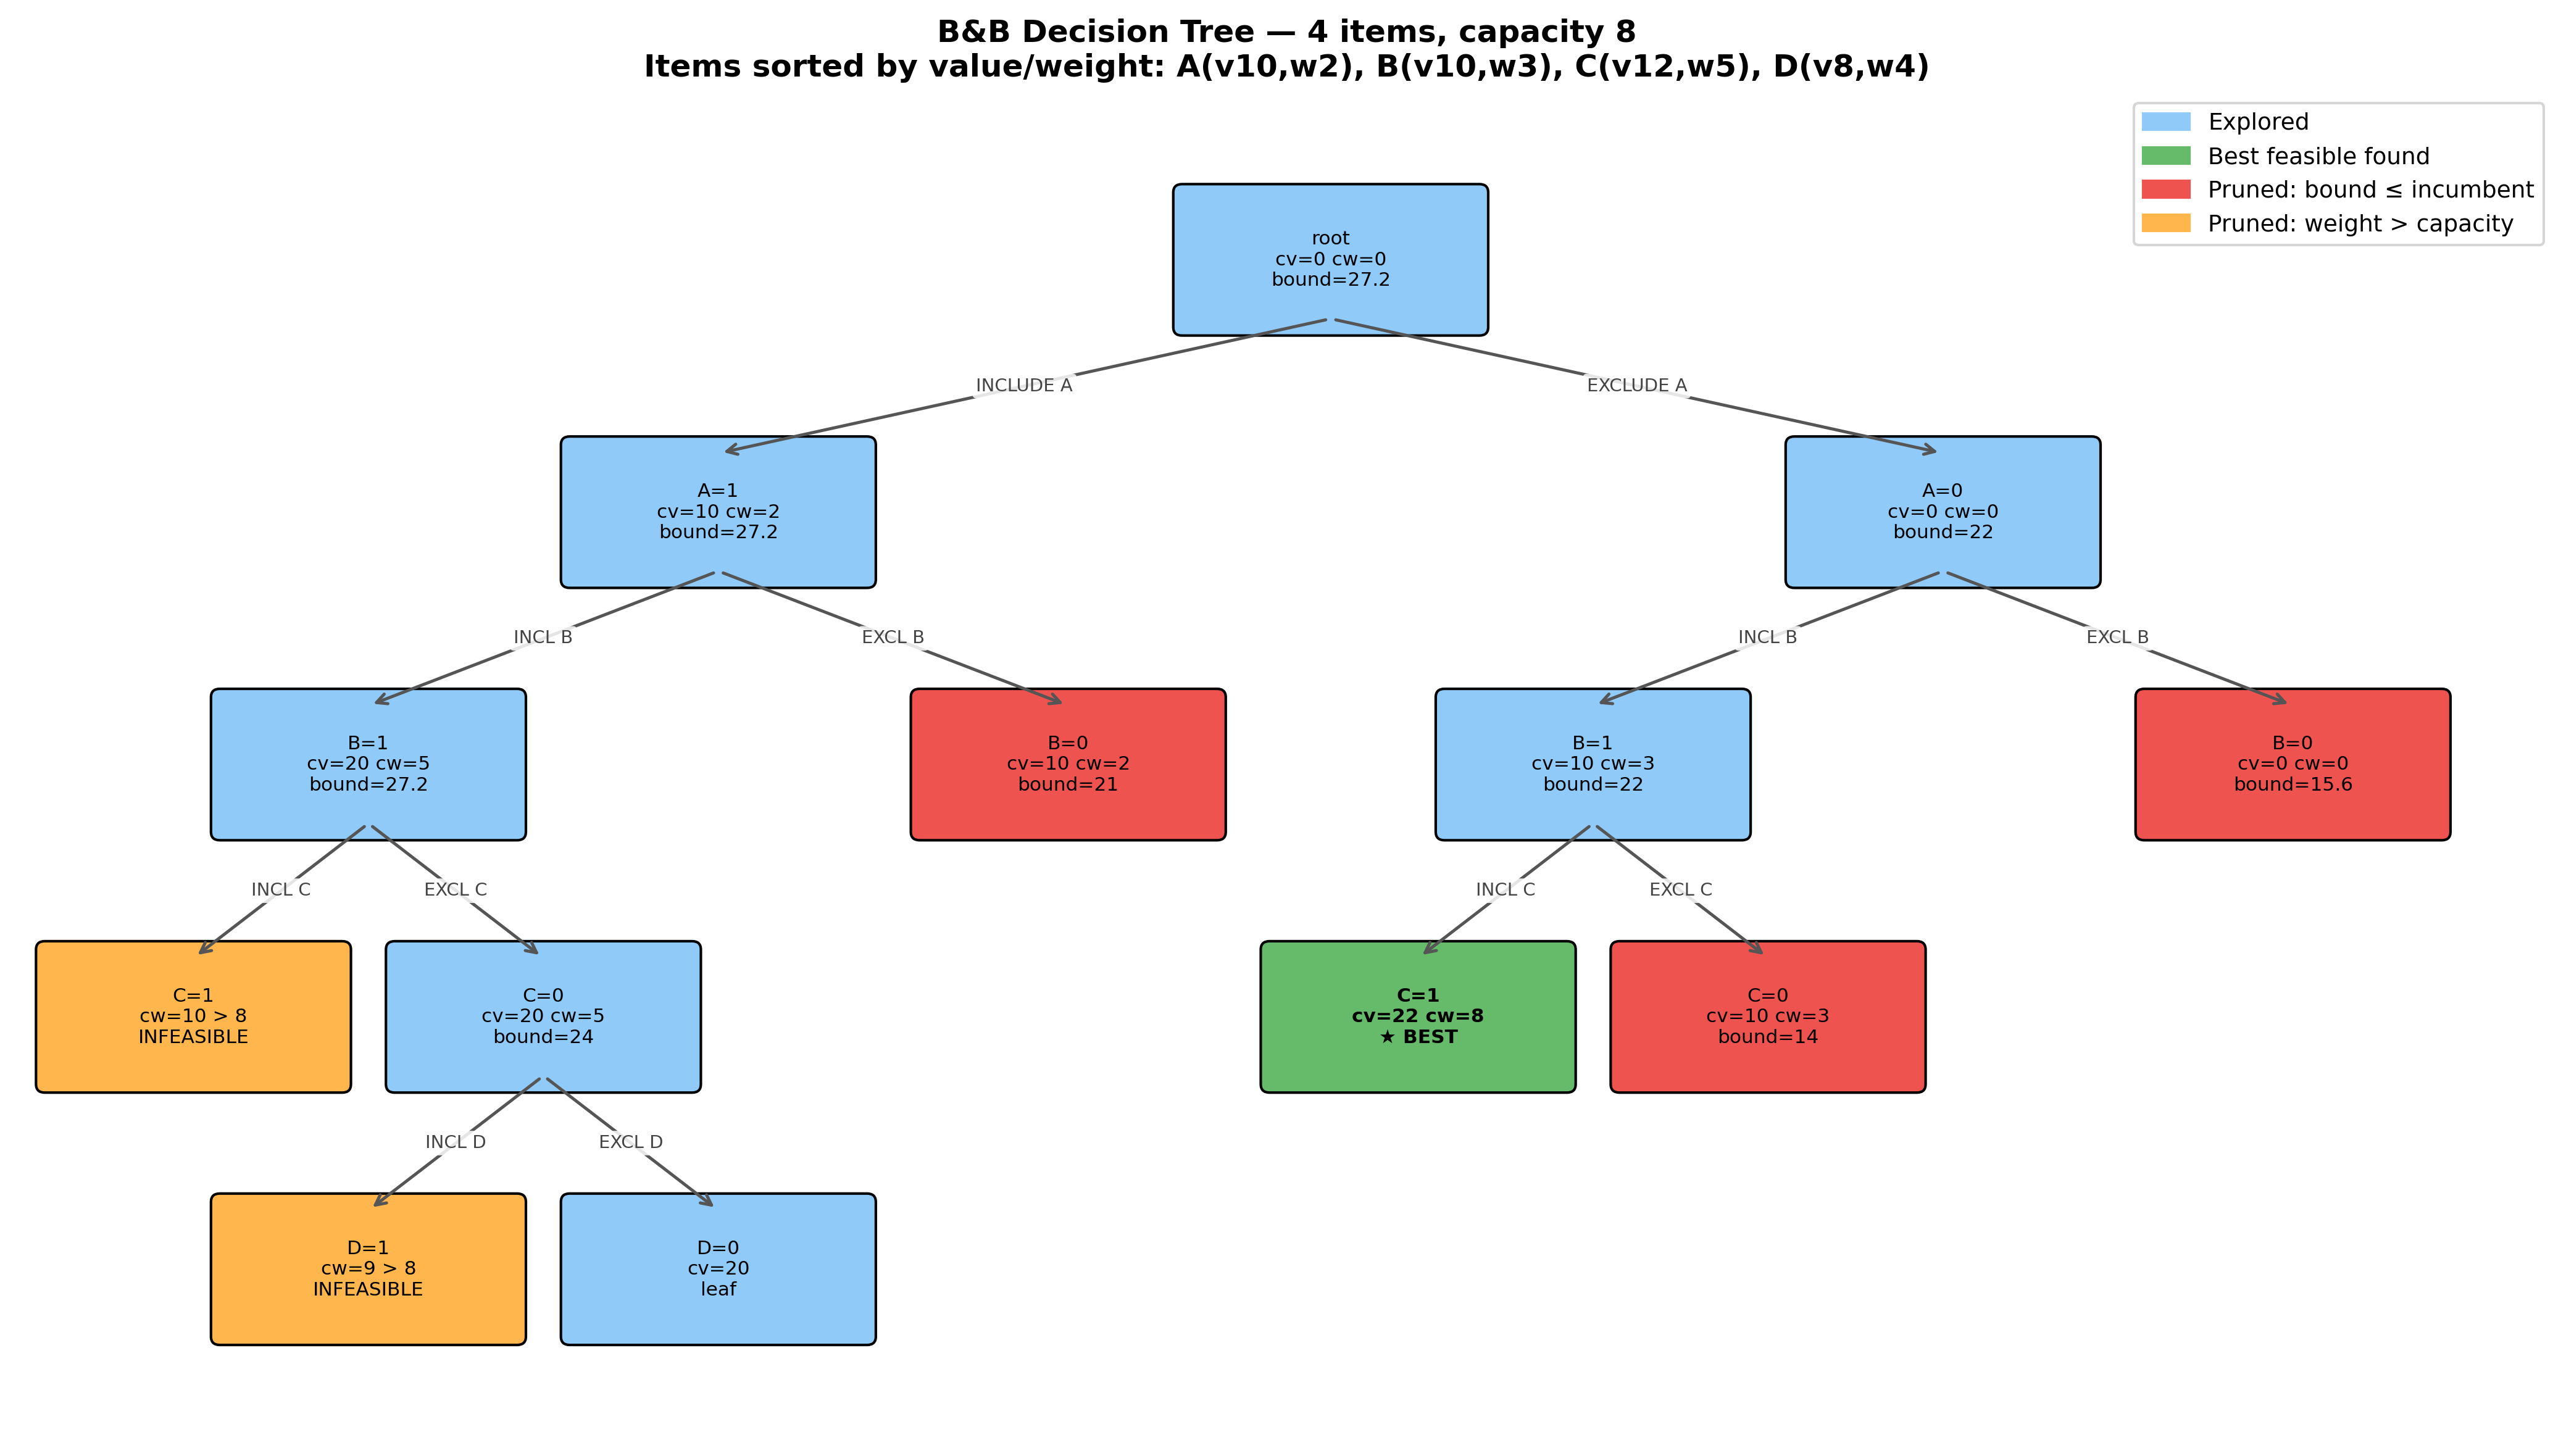
\includegraphics[width=0.80\linewidth]{bb_decision_tree.png}
\end{center}
\figcap{B\&B on a 4-item instance (capacity 8). Of the 16 possible subsets, only \textbf{9 nodes} are visited: 3 pruned by bound, 2 by infeasibility. The optimal subset $\{B, C\}$ with value 22 is found early and powers subsequent pruning.}
\end{posterblock}

% ---------- COLUMN BREAK ----------
\columnbreak

\begin{posterblock}{Methodology}
\textbf{Three-step Branch \& Bound:}
\begin{enumerate}[leftmargin=1.6em,itemsep=4pt,topsep=4pt]
  \item \textbf{Branch.} DFS over include/exclude decisions, ordered by value-to-weight ratio so the greedy guess is tried first.
  \item \textbf{Bound.} LP-relaxation upper bound: a single $O(n)$ greedy sweep.
  \item \textbf{Prune.} Skip any subtree whose bound $\le$ current incumbent.
\end{enumerate}

\vspace{0.4em}
\begin{callout}
The \textit{same} algorithm is implemented in three languages: Python, C++, x86-64 NASM (Win64 ABI, pure integer math, no FPU). The language is the only variable.
\end{callout}

\vspace{0.3em}
\textbf{Pseudocode (C-style)}\\[2pt]
{\ttfamily\small
void branch(int level, int cw, int cv) \{\\
\hspace*{1em}if (cv > best) best = cv;\\
\hspace*{1em}if (level == N) return;\\
\hspace*{1em}if (upper\_bound(level, cw, cv) <= best)\\
\hspace*{2em}return;\hfill\textcolor{BCRed}{// PRUNE}\\
\hspace*{1em}if (cw + W[level] <= CAP)\hfill\textcolor{BCRed}{// INCLUDE}\\
\hspace*{2em}branch(level+1, cw+W[level], cv+V[level]);\\
\hspace*{1em}branch(level+1, cw, cv);\hfill\textcolor{BCRed}{// EXCLUDE}\\
\}\par}
\end{posterblock}

\begin{posterblock}{Model \& Analysis}
The 0-1 knapsack problem is the integer program

\vspace{0.3em}
\begin{callout}
\centering\Large
$\displaystyle
\max \sum_{i=1}^{n} v_i\, x_i
\quad\text{s.t.}\quad
\sum_{i=1}^{n} w_i\, x_i \le C, \quad
x_i \in \{0, 1\}.
$
\end{callout}

The LP relaxation drops $x_i \in \{0,1\}$ in favor of $x_i \in [0, 1]$, producing a tight upper bound: items are sorted by $v_i / w_i$ and packed until the next item exceeds the remaining capacity, taking a fractional slice at the cut. Any partial assignment whose LP bound is $\le$ the current incumbent is pruned, removing entire subtrees from the search.

\vspace{0.5em}
\textbf{Validation Setup}
\begin{itemize}[leftmargin=1.4em,itemsep=4pt,topsep=4pt]
  \item Instance generation: seeded for reproducibility.
  \item Oracle agreement: B\&B output checked against the brute-force optimum on 50 random instances ($n \in [1, 12]$).
  \item Reference solver: PuLP/COIN-CBC on the same instances.
  \item Software stack: Python 3, C++17 (g++ MinGW, static), NASM, PuLP, COIN-CBC.
\end{itemize}
\end{posterblock}

\begin{posterblock}{Implementation \& Tools}
Four solver implementations (Python brute force, plus B\&B in Python, C++, and ASM) are tested against the same canonical instances. The ASM build is statically linked so it can be invoked as a subprocess from the benchmark harness.

\vspace{0.4em}
\renewcommand{\arraystretch}{1.3}
\begin{tabular}{@{}p{0.32\linewidth}p{0.62\linewidth}@{}}
\toprule
\textbf{Component} & \textbf{Tools / Libraries} \\
\midrule
Language       & Python 3.x, C++17, x86-64 NASM (Win64 ABI) \\
Modeling       & PuLP + COIN-CBC \\
Visualization  & matplotlib \\
Build / Test   & g++ MinGW (static), pytest, GNU Make \\
\bottomrule
\end{tabular}
\end{posterblock}

% ---------- COLUMN BREAK ----------
\columnbreak

\begin{posterblock}{Results}
\textbf{Brute force across three languages.} Exponential growth dominates in all three.
\begin{center}

\includegraphics[width=0.66\linewidth]{benchmark_all_three.png}
\end{center}
\figcap{At $n=25$: Python 102\,s, C++ 15.6\,s, ASM 4.9\,s. A faster language helps, but you cannot out-engineer $2^n$.}

\vspace{0.4em}
\textbf{Identical exponential slope, three constants.} Log-linear fits of $T = a\cdot 2^n$ confirm $O(2^n)$ growth across all three brute-force implementations.
\begin{center}
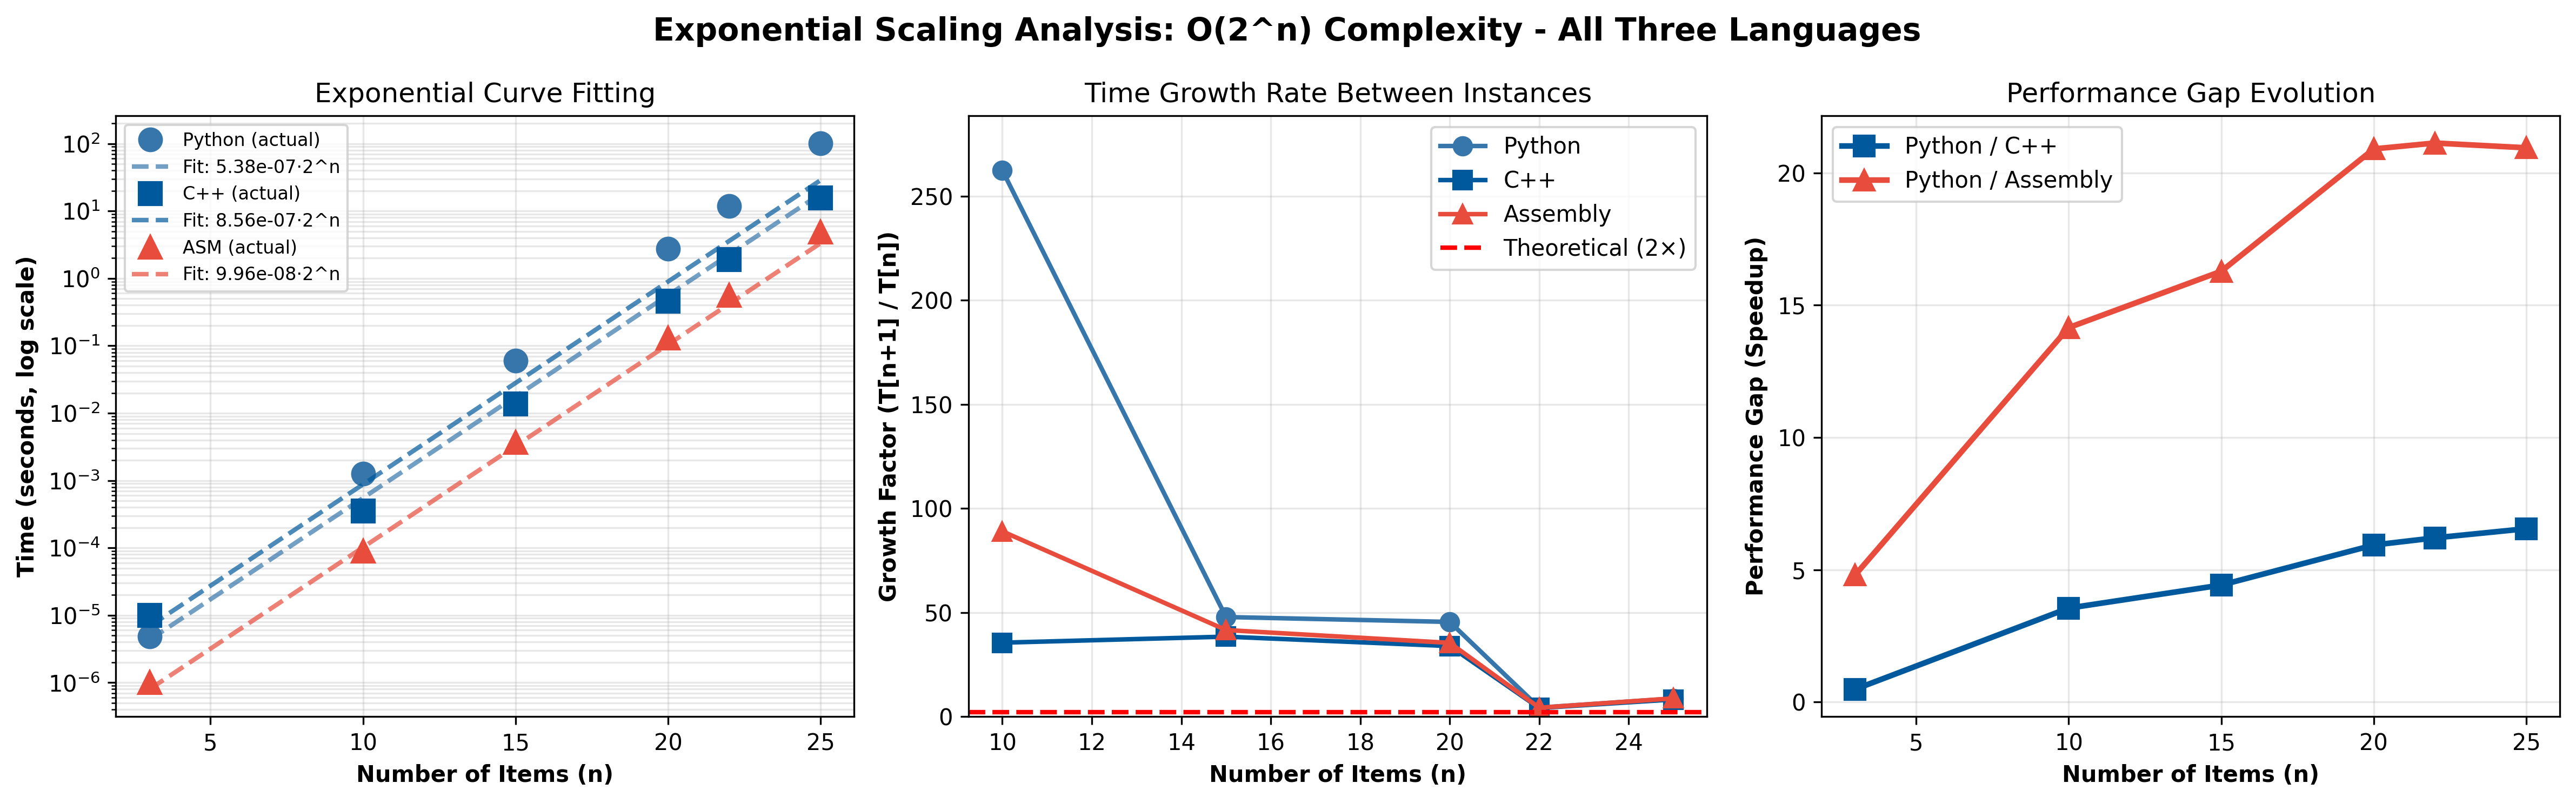
\includegraphics[width=0.70\linewidth]{scaling_all_three.png}
\end{center}
\figcap{The language sets the constant ($a$); it does not change the curve. The ASM $<$ C++ $<$ Python ranking is preserved across the fits. Constant factors compound on exponential work.}

\vspace{0.4em}
\textbf{Same algorithm beats a faster language.} PuLP/CBC (a B\&B engine) is the flat line near the bottom; the three brute-force curves climb past it.
\begin{center}
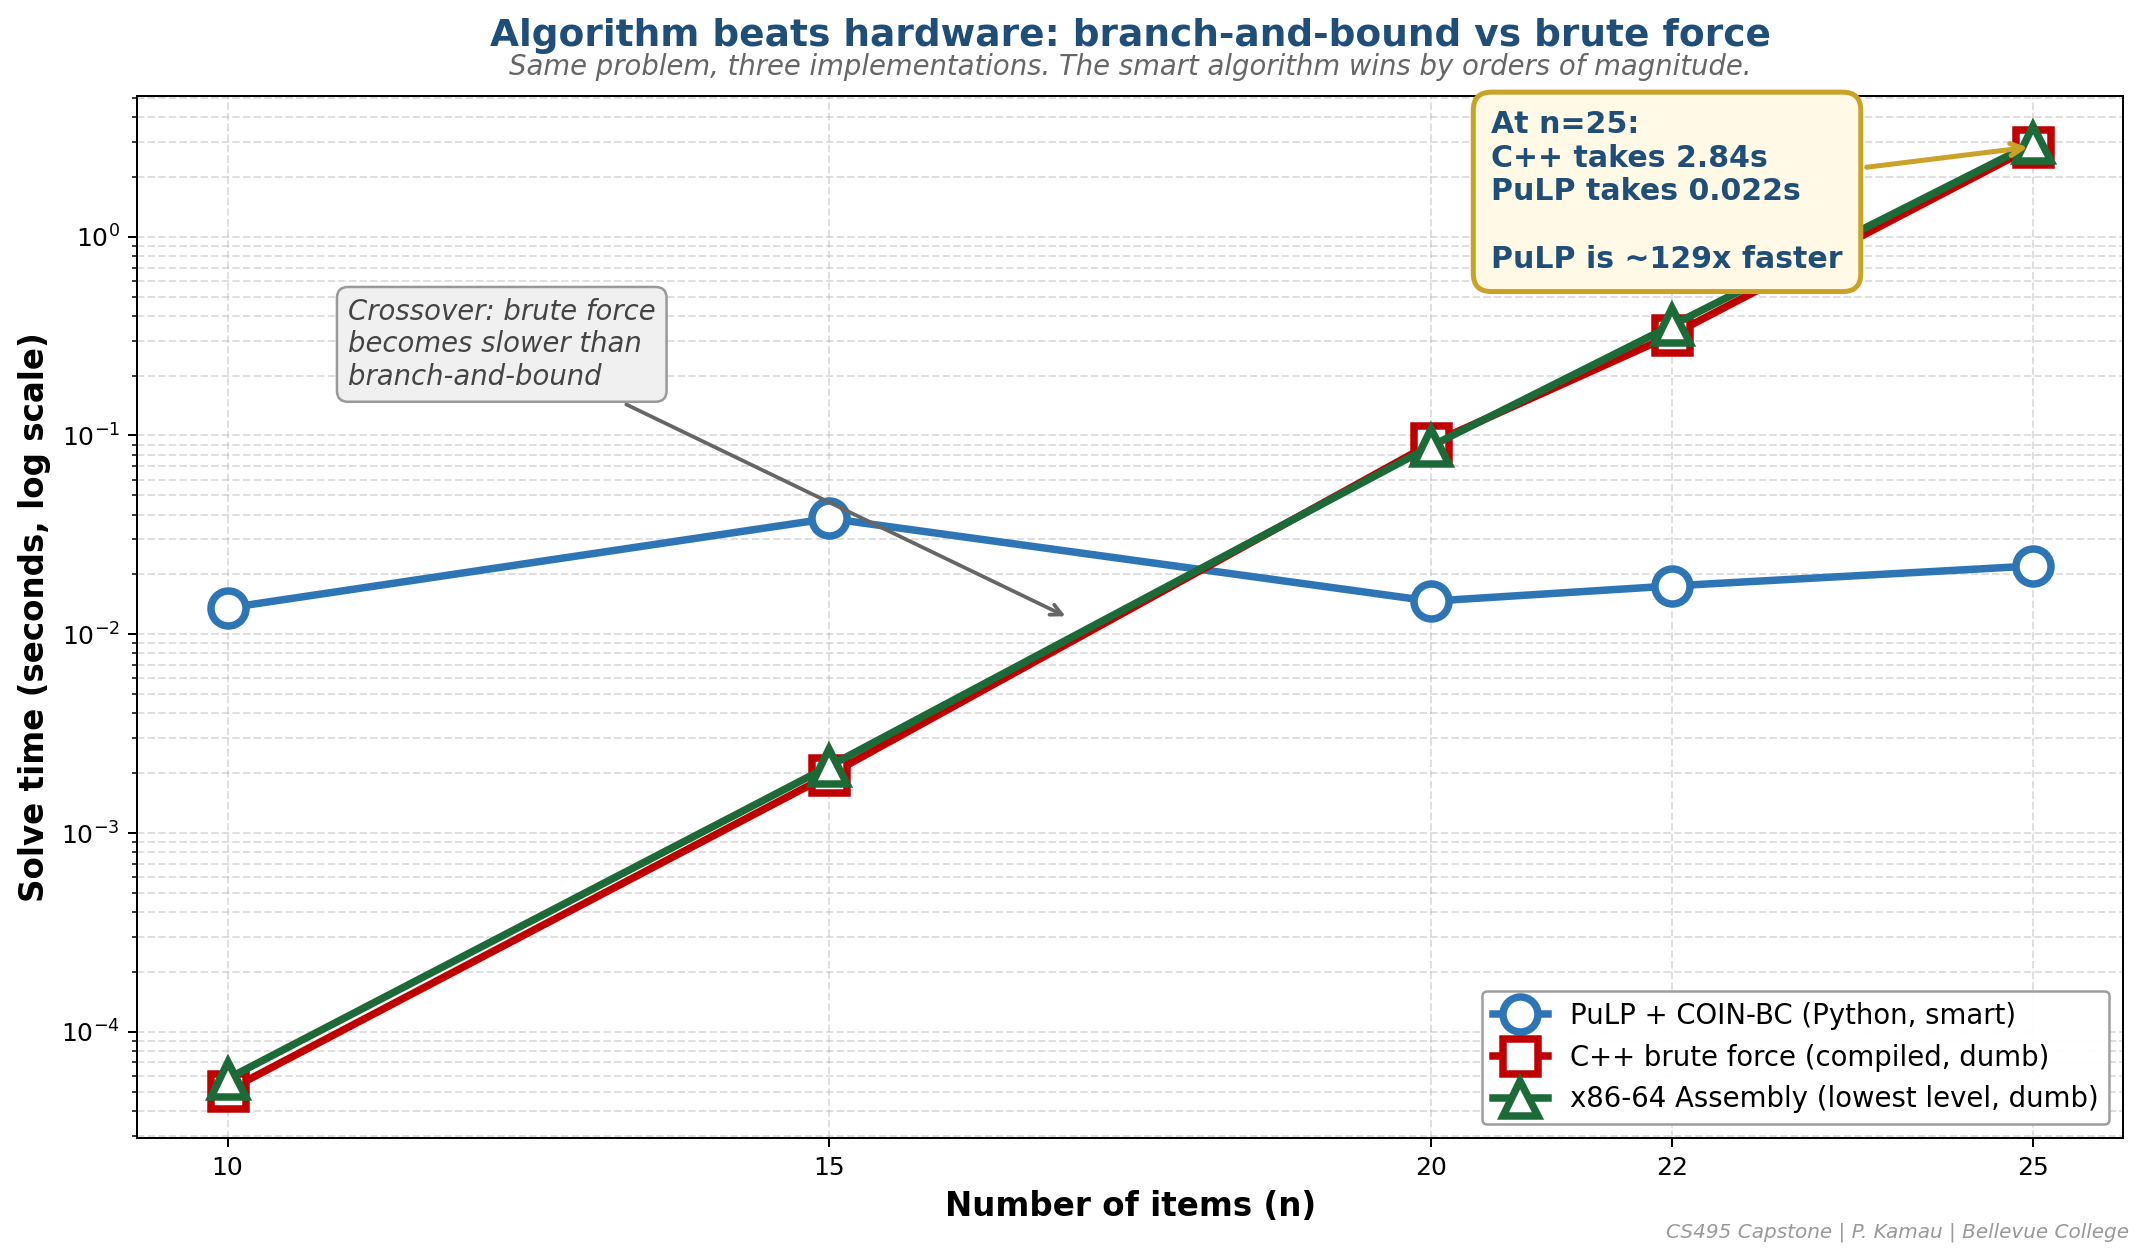
\includegraphics[width=0.66\linewidth]{benchmark_presentation.png}
\end{center}
\figcap{Wall-clock time vs.\ $n$. PuLP/CBC (a B\&B engine) holds flat in milliseconds while all three brute-force curves climb exponentially. Algorithm choice dominates language choice.}

\begin{highlight}
{\bfseries\large At $n = 25$, PuLP/CBC beats ASM brute force by $\sim$170$\times$ and C++ brute force by $\sim$550$\times$.}\\[4pt]
\normalfont\normalsize A smarter algorithm in a slower language beats brute force in the fastest one.
\end{highlight}

\vspace{0.4em}
\textbf{Performance Summary at} \boldmath$n = 25$\unboldmath

\vspace{0.3em}
\renewcommand{\arraystretch}{1.35}
\centering
\begin{tabular}{@{}lrr@{}}
\toprule
\textbf{Solver} & \textbf{Wall time} & \textbf{Speedup vs.\ Python brute} \\
\midrule
Python brute force & 102.22\,s & 1$\times$              \\
C++ brute force    & 15.60\,s  & $\sim$7$\times$        \\
ASM brute force    & 4.88\,s   & $\sim$21$\times$       \\
PuLP/CBC (B\&B)    & 0.028\,s  & $\sim$3{,}650$\times$  \\
\bottomrule
\end{tabular}
\RaggedRight
\end{posterblock}

\begin{posterblock}{Discussion \& Conclusions}
\textbf{Algorithmic choice dominates language choice,} and the two effects compound. A $\sim$10\textsuperscript{6}$\times$ speedup from B\&B dwarfs the $\sim$21$\times$ speedup from a fully hand-coded ASM brute force.

\vspace{0.5em}
\textbf{Key Takeaways}
\begin{itemize}[leftmargin=1.4em,itemsep=4pt,topsep=4pt]
  \item The language ranking (ASM $<$ C++ $<$ Python) is preserved across both algorithms. Constant factors compound on exponential work.
  \item The CBC solver used by PuLP \textit{is} Branch \& Bound; the algorithmic study and the production solver are the same engine.
  \item Cross-solver verification (4 solvers, 9 tests, 50 random instances) caught no disagreements after the algorithm was finalized.
\end{itemize}

\vspace{0.3em}
\textbf{Limitations:} synthetic instances only; $n$ capped at 25 because brute force becomes infeasible past that point; B\&B wall-clock time is instance-specific, not monotone in $n$ (e.g., $n = 22$ ran faster than $n = 20$ in our trials).

\vspace{0.3em}
\textbf{Future Work:} LLM-generated-solver comparison using this verification harness as ground truth.
\end{posterblock}

\begin{posterblock}{References}
\footnotesize
\begin{enumerate}[leftmargin=1.4em,itemsep=1pt,topsep=2pt]
  \item Land, A.\,H.\ \& Doig, A.\,G.\ (1960). An automatic method for solving discrete programming problems. \textit{Econometrica} 28(3), 497--520.
  \item Dantzig, G.\,B.\ (1957). Discrete-variable extremum problems. \textit{Operations Research} 5(2), 266--277.
  \item Kellerer, H., Pferschy, U.\ \& Pisinger, D.\ (2004). \textit{Knapsack Problems.} Springer.
  \item Pisinger, D.\ (1997). A minimal algorithm for the 0-1 knapsack problem. \textit{Operations Research} 45(5), 758--767.
  \item Forrest, J.\,J.\ \& Lougee-Heimer, R.\ (2005). \textit{CBC user guide.} INFORMS Tutorials.
  \item Mitchell, S., O'Sullivan, M.\ \& Dunning, I.\ (2011). PuLP: A linear programming toolkit for Python.
\end{enumerate}
\vspace{0.3em}
\textit{Acknowledgments:} thanks to \textbf{Dr.~Pedro Albuquerque} and the Bellevue College CS program. \textbf{Contact:} pm.kamau24@gmail.com \;\textbar\; \textbf{Code:} github.com/PeterKamau24/CS495-Logistics-Optimization-LLM
\normalsize
\end{posterblock}

\end{multicols}

\end{document}
